% Conclusions

\chapter{Discussion and Conclusion}

In this chapter, the results and analyses from the experiments is deliberated to pull a reasonable explanation for the phenomenon. Limitations and challenges from the experiments are examined as well. After that, some recommendations for further empirical study on the subject is going to be suggested. Last but not least, conclusion of the thesis project and possibility to commercialize Voxer are drawn.

\section{Discussion}

In empty pipe, the introduced flow is concentrated around the center region while the flow near the inner wall is affected by \gls{noslip}. Meanwhile, Voxer disperses the flow to the wall. As observed from the result of both experiments, we can clearly recognize that having Voxer 40$^{\circ}$ in any position within the pipeline led to a larger raise in pressure losses than Voxer 30$^{\circ}$. This could be explained by the dimension difference between two kinds of elliptical shape. The y-axis radius of Voxer 40$^{\circ}$ is much shorter than Voxer 30$^{\circ}$  (see figure \vref{fig:twovox}) so the vorticity magnitude after Voxer 40$^{\circ}$ is also shorter. 
\begin{wrapfigure}{r}{0.4\textwidth}
  \begin{center}
    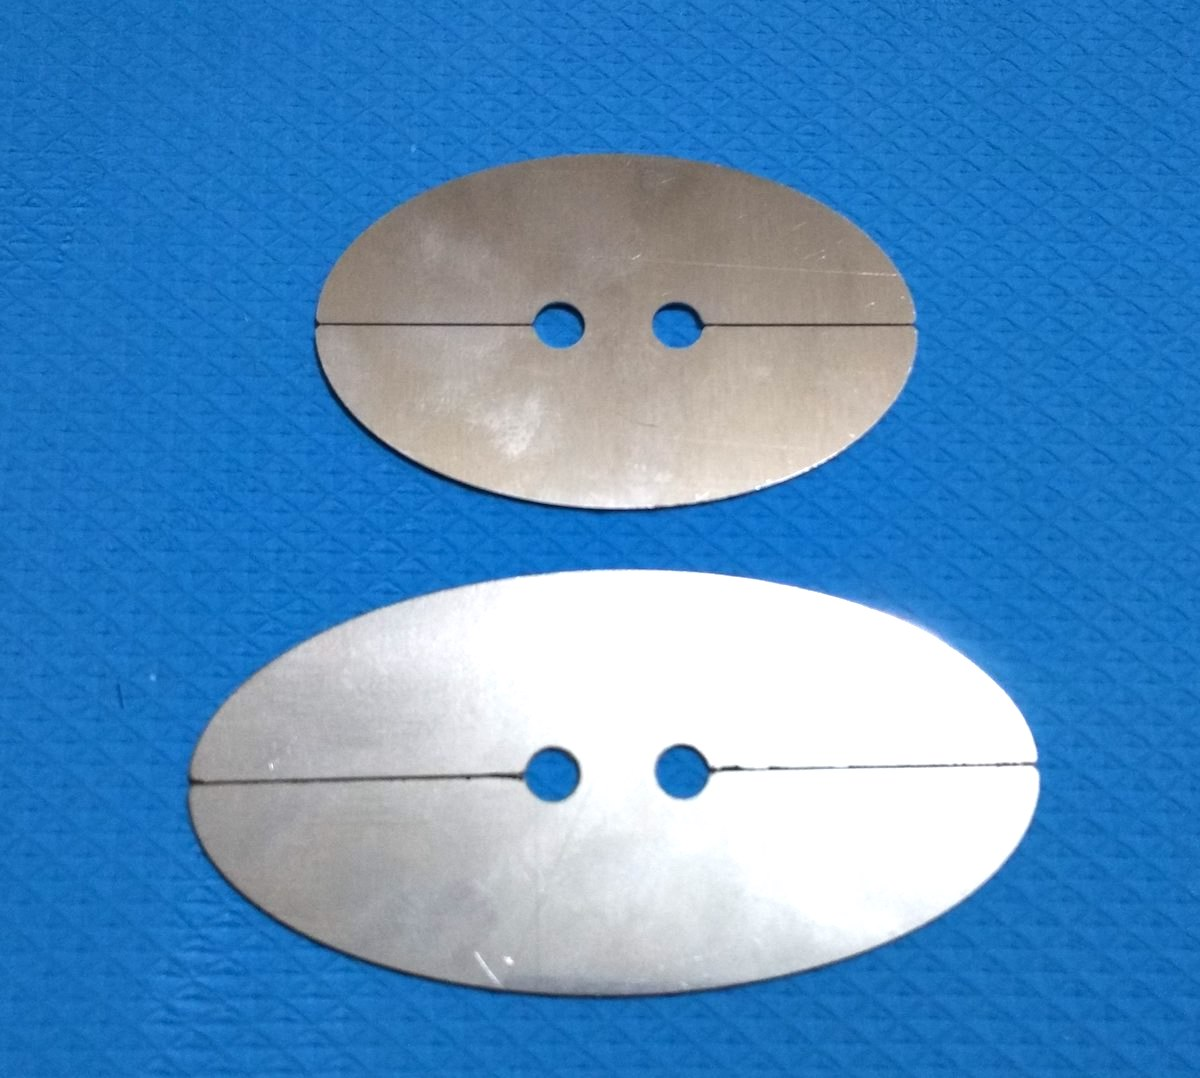
\includegraphics[width=0.38\textwidth]{twovoxers}
  \end{center}
  \caption{Unbended Voxer 40$^{\circ}$ (up) and Voxer 30$^{\circ}$ (down)}
  \label{fig:twovox}
\end{wrapfigure}
The shorter vorticity magnitude corresponded to higher frequency which led to higher pressure \cite{scz:article}. The appearance of Voxer 40$^{\circ}$ in mixed combination of 2 types of Voxer showed the impact of shorter vorticity magnitude on pipe pressure.

In the laboratory experiment, the contraction of sectional and total pressure losses by a single Voxer always occurs steadily in the pipelines. It can be said that each Voxer has a nominal resistance and loss reduction. With the presence of many Voxers is series, this can be agued that there were more flow resistance than loss reduction in the piping section. The first Voxer had already resulted in larger loss reduction than resistance but the following Voxers have no loss reduction because the vortex current had already been generated by the first Voxer. With the short distance between each Voxer in those combinations having more than 2 Voxers, the introduced flow wasn't completely developed before meeting the next Voxer. That Voxer became a nuisance to the water flow. Therefore, while Its nominal resistance stayed constant, the total and larger sectional pressure difference is higher. 
However, we should also consider the bend at the outflow which caused strong turbulence at the end of pipeline which might have increased a small amount of total pressure difference in those combinations having only the first Voxer before the starting elbow. The first Voxer reduces energy consumption in the pipe but the ending curve at the large distance raises pressure drop. That might be a good reason for putting the second Voxer before the ending curve (combination V14 - Voxer 30$^{\circ}$), as recommended in the technical document \cite{voxer:article}, to support loss reduction in the curved pipe. The performance of this combination was recorded as the best combination in the lab experiment. 

In Keravan experiment, since the condition was uncontrolled by many minor incidents and outside factors, the evaluation must proceed in cautious approach to avoid overconfident conclusion. From all data collected in the experiment, especially the one illustrated in figure \ref{fig:pabdensity}, the difference of total pressure losses among empty pipe, Voxer 40$^{\circ}$ and Voxer 30$^{\circ}$ is very distinct. This can be explained by the disproportionation between loss reduction and resistance that was mentioned before. Looking to the sectional pressure change, which is shown in figure \ref{fig:pbdensity}, we can determine that Voxer 30$^{\circ}$ has a capability to cut down energy consumptions. Since the graph has shown that Voxer 30$^{\circ}$ has many values which are equal or even lower to values of the sectional pressure loss in the empty pipe. 

\section{Limitations and Recommendations}

There are still many limitations in out study about Voxer which are mainly related to methodology and equipments. In our experiments, we connected the pressure meter to the pipelines by measuring hose attached to a connector which doesn't have direct contact with internal flow around central region. It is doubting that these measuring points are only capable of measuring static pressure but not stagnation pressure. The original needles \cite{danfoss:web} attached to measuring hoses might result better performance in measuring pressure drop. Since this is only a cautious thinking, it would be better to have access to other measuring instruments to compare in order to ensure the better result. 

The model of relationship between pressure loss and Voxer's angle can be established by using the method of repeating variables (p308) \cite{cengel:book}. Since the data size from comparative testing was quite restriced and depending on many outside factors, more data from more diverse combinations can be analysed by building stimulation model of Voxer in pipeline by using \gls{cfd}. Without limitations of time and resources, further research in the future can utilize \gls{cfd} to perform better stimulation analysis of vortex flow by defining correct boundaries, fluid properties, model mesh and related mathematical equations. 

\section{Conclusion}

Comparative measurements were performed to investigate the effect of Voxer wing of \gls{ltd} on reducing energy consumptions in water cooling piping section at Keravan Energy Ltd. The sectional and total pressure difference of the pipelines can be slightly reduced by placing a Voxer before the 90$^{\circ}$ curve at the end of piping section. This conclusion is cautiously drawn as it matches the product placement suggestion from \gls{ltd}.  Voxer can be introduced to the market with careful planning of product customization and position in customer's system. 

\clearpage %force the next chapter to start on a new page. Keep that as the last line of your chapter!
